%\documentclass[draft]{ws-procs9x6}
\documentclass{ws-procs9x6}
\usepackage{comment}
\usepackage{subfigure}
\usepackage{color}

\begin{document}

\title{Bridging the gap: improving local multiple alignment with a novel heuristic for gapped extension.}

\author{Todd J. Treangen$^\dag*$}

\address{Dept. of Computer Science, Technical Univ. of Catalonia\\
Barcelona, Spain\\
$^*$E-mail: treangen@lsi.upc.edu}

\author{Aaron E. Darling$^\dag*$}

\address{Institute for Molecular Bioscience, Univ. of Queensland\\
Brisbane, Australia\\
$^*$E-mail: a.darling@imb.uq.edu.au}


\author{Guillaume Achaz}
\address{Atelier de Bioinformatique, Univ. Pierre et Marie Curie-Paris 6,\\
 Paris, France}

\author{ Mark A. Ragan}

\address{Institute for Molecular Bioscience, Univ. of Queensland\\
Brisbane, Australia\\
}

\author{ Xavier Messeguer}

\address{Dept. of Computer Science, Technical Univ. of Catalonia\\
Barcelona, Spain\\
}

{\center \scriptsize $^\dag$ These authors contributed equally to this work \\}

\begin{abstract}
The identification of homologous DNA via sequence alignment is a basic building block in comparative genomics.  We present a method for accurately and sensitively identifying homologous DNA sequence in multiple genomes. Our method is based around an efficient heuristic for local multiple alignment, featuring a novel method for gapped extensions. In practice, we are able to sensitively identify conserved, potentially repetitive, regions in one or more DNA sequences.
\end{abstract}

\keywords{sequence alignment}


\bodymatter

\section{Introduction}

The importance of accurate homology identification to comparative genomics can not be underestimated~\cite{Kumar07}. To date, pairwise local sequence alignment methods~\cite{ref-blastz, ref-ssearch} have been the prevailing technique to identify homologous nucleotides.  When more than two copies of a homologous sequence element are present in the data, pairwise homology detection methods generate a listing of all possible pairs of homologous elements.  Apart from the obvious inefficiency of considering all pairwise homology relationships, a collection of pairwise alignments is not ideal because they are rarely amenable to comparative genomic and phylogenetic analysis without further processing into a multiple alignment.

Local pairwise alignments can be merged to create a multiple alignment by a variety of methods~\cite{ref-tba,ref-aba,ref-dialign,ref-related1}. Such methods commonly assume that pairwise homology relationships are transitive, such that if nucleotide $a$ is homologous to nucleotide $b$, and $b$ is to $c$, then $a$ must also be homologous to $c$.  Thus, in order to merge pairwise alignments, such methods must tackle the challenging problem of resolving inconsistent transitive homology relationships.  Multiple alignment has been demonstrated to be more accurate than pairwise alignment, especially when dealing with a large number of divergent sequences~\cite{ref-mlagan,ref-aubergene}.  As the number of homologous sequences grows, we might expect that the number of inconsistent relationships in a collection of pairwise alignments would grow quadratically, whereas a direct multiple alignment method would provide an increasingly accurate alignment.  Highly repetitive regions in the input sequences can cause serious efficiency problems for pairwise methods, as they create $O(r^{2})$ pairwise alignments in the presence of a repeat with $r$ copies.  Mammalian Alu repeats and IS elements in microbes are two common examples of the overwhelming abundance of repetitive sequence in naturally occurring genomes.

Local multiple alignment has the inherent potential to avoid pitfalls associated with pairwise alignment. Although optimal multiple alignment under the SP objective function remains intractable~\cite{ref-wangjiang}, progressive alignment heuristics offer excellent speed and accuracy~\cite{ref-clustalw, ref-tcoffee} especially when combined with tree-independent iterative refinement~\cite{ref-muscle}, or probabilistic consistency measures~\cite{ref-probcons}. Rather than merging pairwise alignments, why not exploit years of research into multiple alignment heuristics by directly constructing a multiple alignment? We aim to bridge the gap in efficiency by presenting a novel heuristic for gapped extension for sensitive local multiple alignment. \textbf{It's not just a gap in efficiency, is it?  I think we're automatically creating a type of alignment that wasn't previously possible...}

%In the context of \textit{local} multiple alignment, the fundamental problem with such an approach is that current methods for progressive %alignment with iterative refinement compute \textit{global} alignments, i.e. they implicitly assume that input sequences are homologous over %their entire length.

%Thus, our aim is to avoid this problem and at the same time bridge this gap in efficiency by presenting a novel heuristic for gapped extension %for sensitive local multiple alignment.

\section{A heuristic for local multiple alignment}
We present a novel heuristic for directly computing local multiple alignments that exploits the MUSCLE multiple alignment algorithm to compute gapped extensions of seed matches (see Figure~\ref{fig-main}). Gapped alignments arise when to extending seeds to fully capture surrounding sequence homology. Our method assumes that a fixed number of nucleotides flanking a seed match is likely to be homologous and computes a global multiple alignment on the flanking region.  In some cases our assumption of flanking homology proves erroneous and results in an alignment of unrelated sequences.  We use a hidden Markov model to detect any such non-homologous regions embedded in the global multiple alignment.  Non-homologous regions are then removed from the alignment and the local-multiple alignment is trimmed to reflect the updated boundaries of homology.  Finally, we present an approximation method to assign statistical significance to the resulting local-multiple alignments.

\begin{figure}[p]
\begin{center}
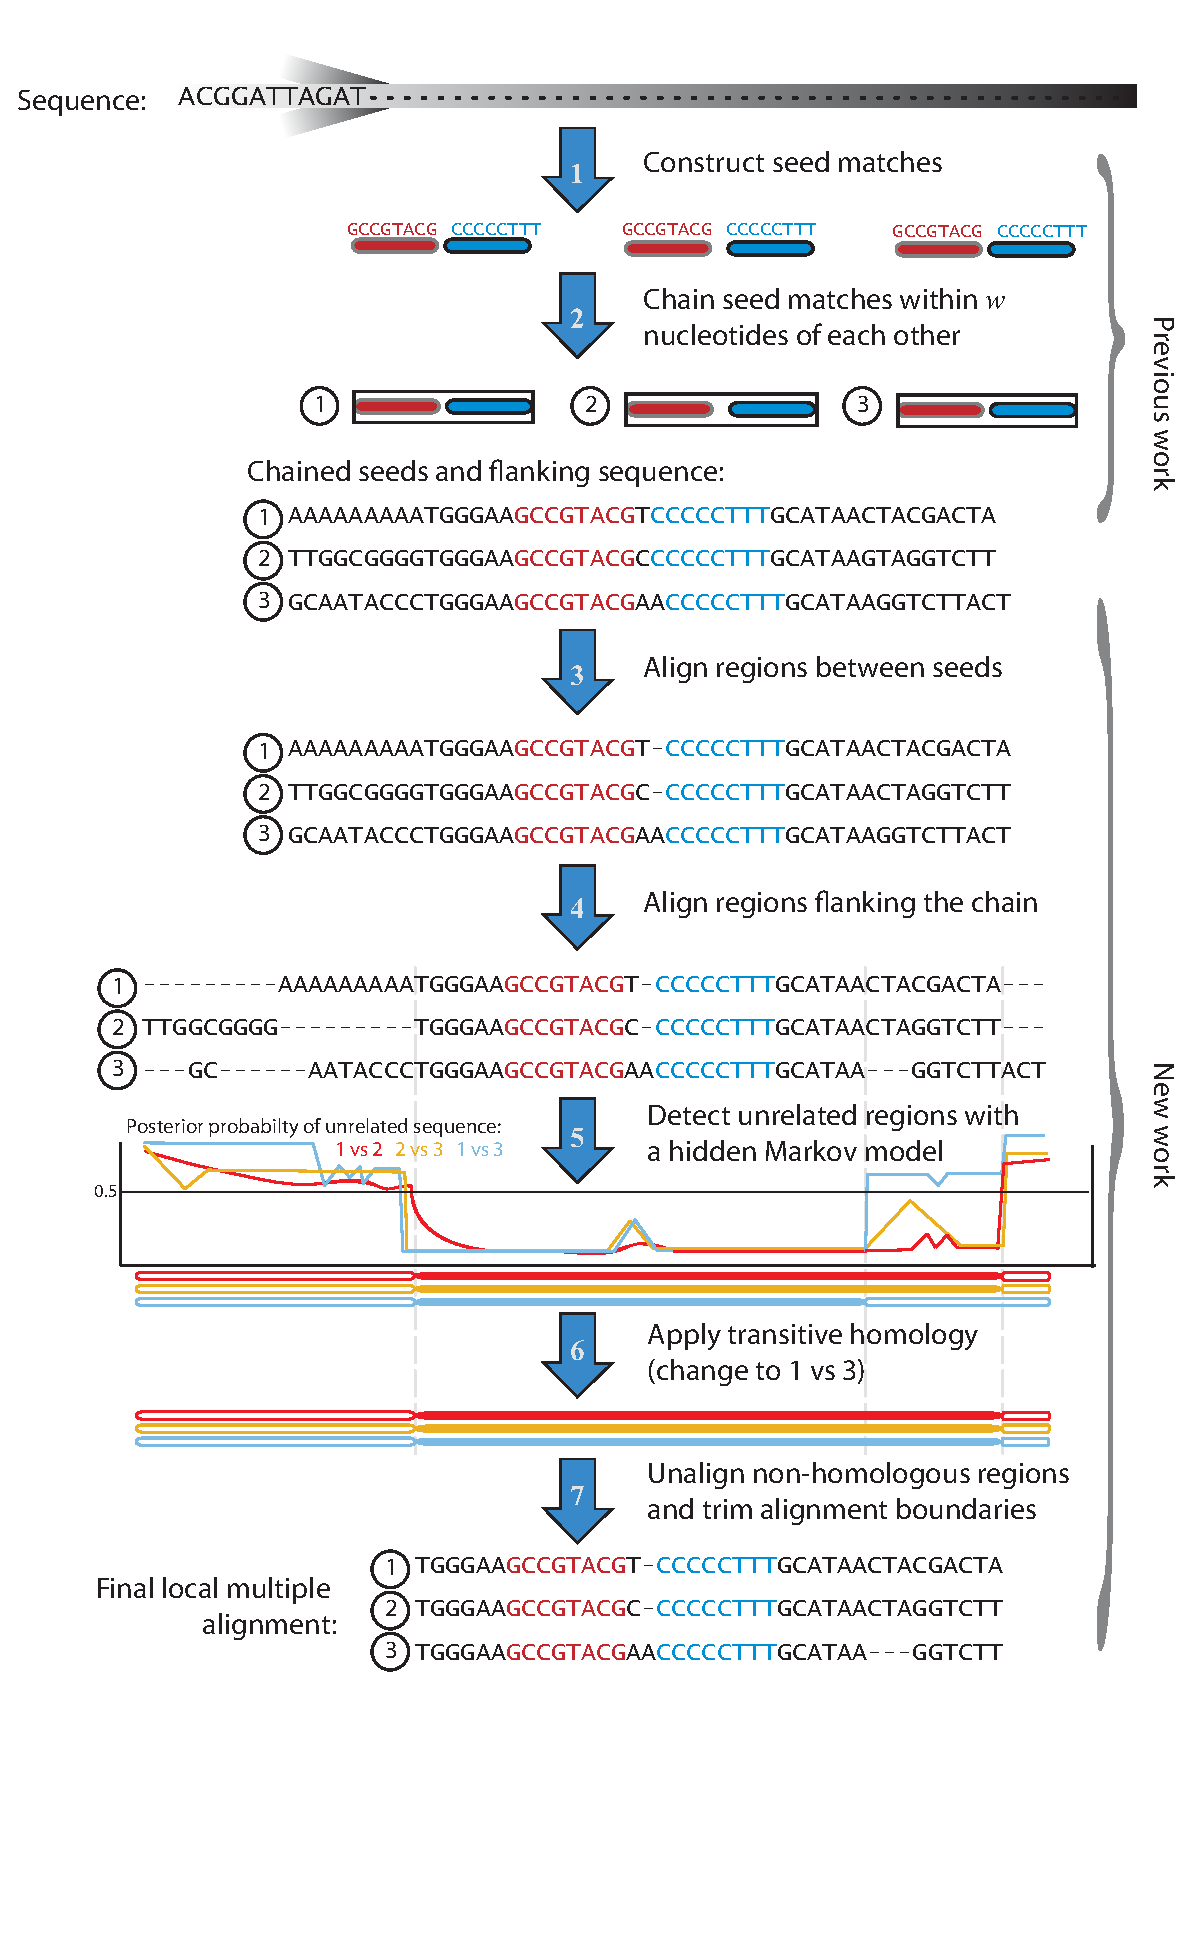
\epsfig{file=./figures/extension.eps,width=4.0in}
%\subfigure[Visual representation of our algorithm]{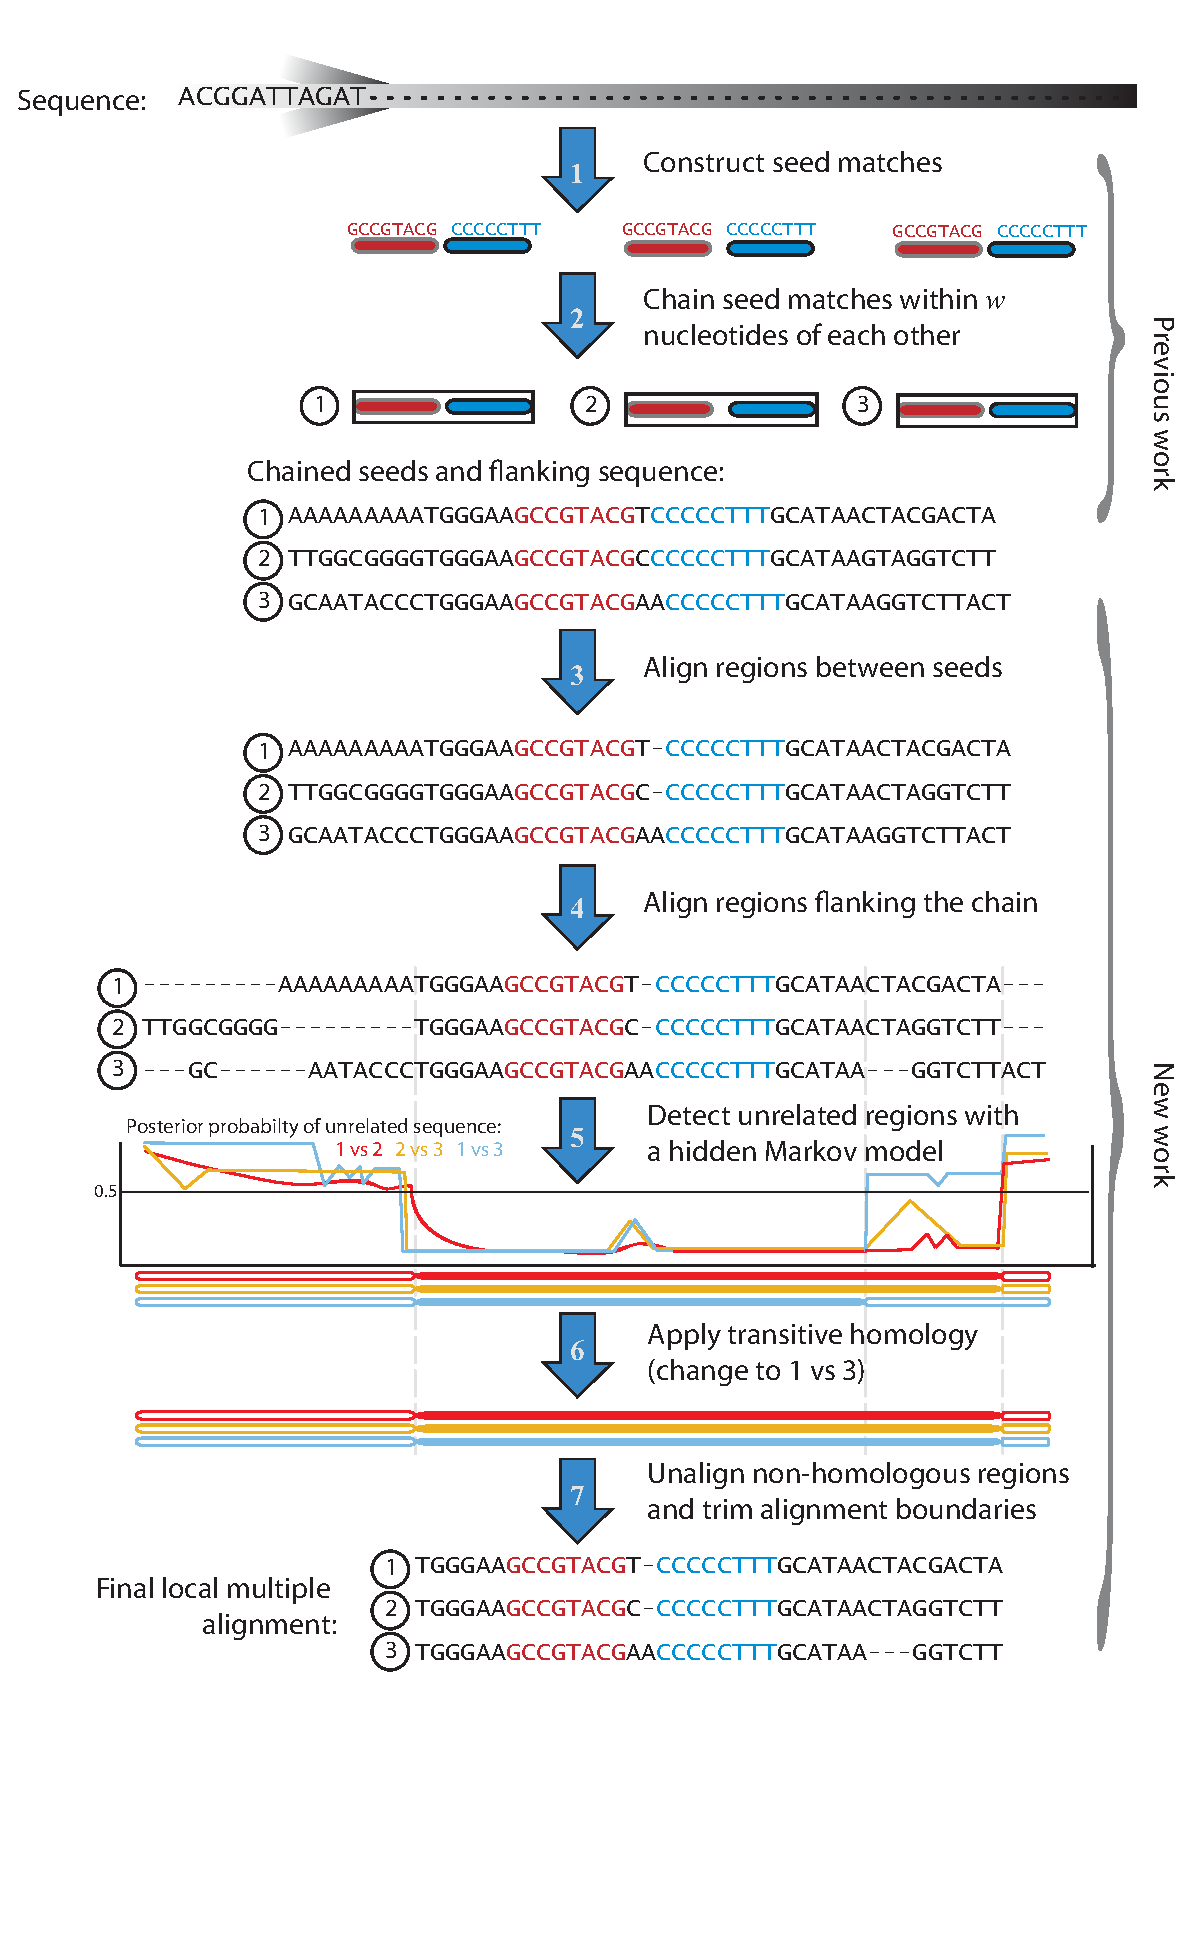
\epsfig{file=./figures/extension.eps,width=3.0in}}
%\subfigure[Flowchart of the algorithmic process ]{ 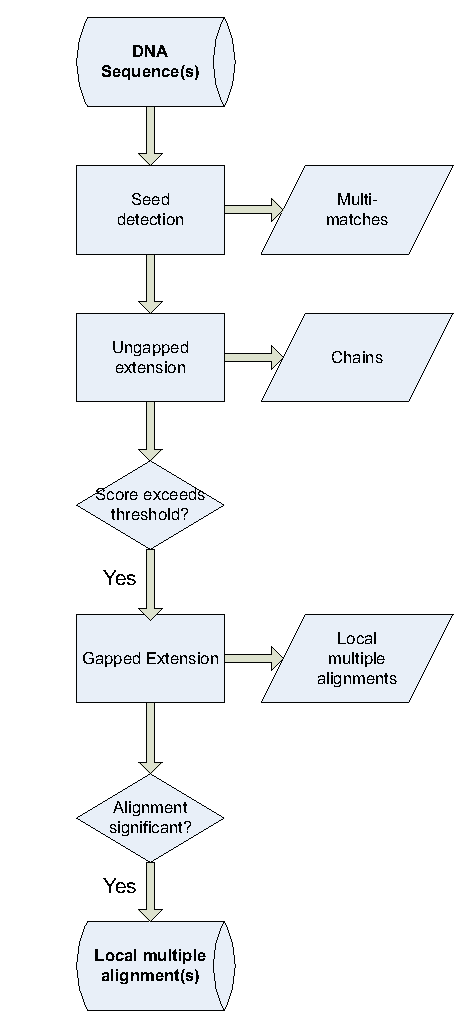
\epsfig{file=./figures/flowchart.eps,width=1.7in}}
\end{center}
\caption{Overview of the method, starting with an input sequence and ending with a set of local multiple alignments. First we (1) detect multi-matches in input sequence(s) using palindromic spaced seeds, then we perform (2) prioritized chaining of all multi-matches.  The resulting chain contains two matches and three match components labeled 1, 2, and 3.  We then perform gapped alignment of the region between chained matches (3).   In step (4), we perform a gapped extension by computing a global multiple alignment on the regions to the left and right of each chain component.  The resulting alignment may contain non-homologous sequence, so in step (5) we apply a Hidden Markov Model to detect the poorly aligned regions indicative of unrelated sequence.  In step (5), heavily diverged homologous sequences may be incorrectly classified as nonhomologous. The posterior probability of being in the non-homologous state for each alignment column is shown.  Step (6) computes transitive homology relationships to ensure a consistent alignment and aid detection of divergent homologous sequences.  Finally, in step (7) we unalign regions found to be non-homologous.  If we find after step (7) that the alignment boundaries have been extended, we acquire additional flanking sequence and return to step (4) for another round of extension.}
\label{fig-main}
\end{figure}


%\colorbox[named]{Gray}{adfa}

\subsection{Extracting multi-matches from the input sequence}

Given a sequence $\mathcal{S}=s_1, s_2,\dots, s_N$ of length $N$
defined over an alphabet $\{A,C,G,T\}$, our goal is to identify all
significant local multiple alignments on subsequences of $\mathcal{S}$. Our
proposed method first extracts candidate ungapped alignments, or multi-matches,
among subsequences in $\mathcal{S}$, denoted as $\mathbf{M}$. To extract multi-matches from the input sequence, we utilize a palindromic spaced seed pattern, which is analyzed at each position in the input sequence.  Previously we have demonstrated that palindromic spaced seeds offer good efficiency and reasonable sensitivity on a variety of input sequences~\cite{ref-procrast}.

We refer the number of matching regions in $\mathcal{S}$
by a given match $M_i \in \mathbf{M}$ as the
\textit{multiplicity} of $M_i$, denoted as $|M_i|$. We refer to each
matching region of $M_i$ as a \textit{component} of $M_i$. Note that
$|M_i| \geq 2~\forall~M \in \mathbf{M}$.  We denote the left-end
coordinates in $\mathcal{S}$ of each component of $M_i$ as $M_i.L_1,
M_i.L_2,\dots, M_i.L_{|M_i|}$, and similarly we denote the right-end
coordinates as $M_i.R_x$.  When aligning DNA sequences, matches may
occur on the forward or reverse complement strands. To account for
this phenomenon we add an orientation value to each matching region:
$M_i.O_x \in \{1,-1\}$, where 1 indicates a forward strand match and
-1 for reverse.

Our algorithm has an important limitation on the matches in
$\mathbf{M}$: no two matches $M_i$ and $M_j$ may have the same
left-end coordinate, e.g. $M_i.L_x \neq M_j.L_y~\forall~i, j, x, y$
except for the identity case when $i=j$ and $x=y$.  This constraint
has been referred to by others as \textit{consistency} and
\textit{transitivity}~\cite{ref-transitivity} of matches.  In the
present work we only require consistency and transitivity of matches
longer than the seed length, e.g. seed matches may overlap.

\subsection{Creating chains of multi-matches}

Once a list of multi-matches has been generated, we employ an efficient chaining algorithm to identify overlapping and nested chains of multi-matches~\cite{ref-procrast}. A brief review of the method follows.
In order to chain over each region of sequence $\mathcal{O}(1)$ times,
the method chains matches in order of decreasing multiplicity--we
extend the highest multiplicity matches first. We first chain all matches
with the same multiplicity within $w$
characters. When a match can no
longer be chained without including a gap larger than $w$
characters, our method identifies the neighboring \textit{subset}
matches within $w$ characters. We then \textit{link} each
neighboring subset match to the chained match. We refer to the
chained match as a \textit{superset} match. Rather than immediately
extend the subset match(es), we \textit{procrastinate} and extend
the subset match later when it has the highest multiplicity of any
match waiting to be extended. When chaining a match with a linked
superset, we immediately include the entire region covered by the linked superset
match--eliminating the need to re-examine sequence already covered by
a previous match extension.

\subsection{Gapped extension of high scoring chains}

After successful chaining of multi-matches, we perform gapped alignment on all collinear regions located between two adjacent components to generate unextended local multiple alignments. \textbf{Not after all chains, but during each chain's extension.}   \textbf{((}We first evaluate the chain in order make a decision whether its worth spending computational resources on gapped extension. We can require that two seeds were present in the chain, allowing lower seed sizes $k$ to be used. This idea has been used in other local alignment heuristics~\cite{ref-blastz,ref-gappedblast,ref-blat} in order to minimize the number of gapped extensions that do not improve the boundaries of the chain.\textbf{)) can this be shortened to one sentence since it's not a new idea?}

To perform a gapped extension in each direction, we use MUSCLE to align the left/right region immediately surrounding the unextended local multiple alignments. The size of the extension window we send to MUSCLE is determined empirically to optimize efficiency and sensitivity. \textbf{FIXME.  this may be a new enough idea to warrant writing the equation into the text.}

\subsubsection{Identifying non-homologous regions}
\begin{figure}[t]
\centering 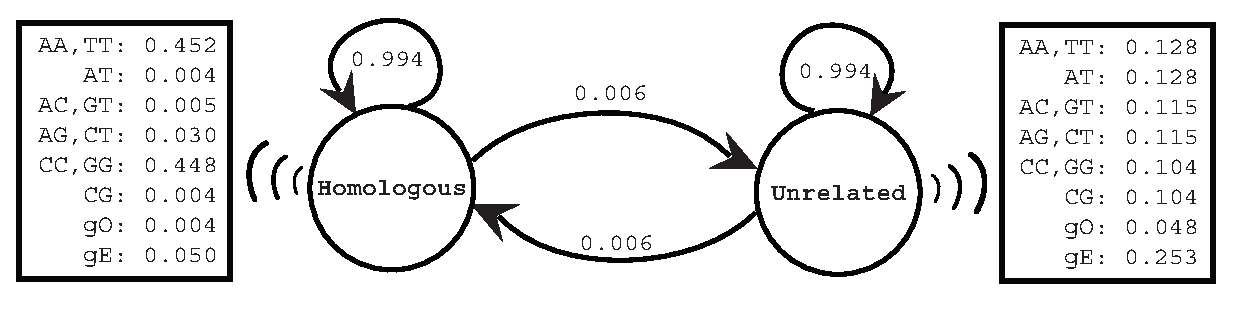
\epsfig{file=./figures/hmm.eps,width=4.5in}
\caption{Hidden Markov model used to detect pairwise alignments of unrelated sequence. The HMM has states which model alignment columns containing homologous and unrelated sequence.  Emissions correspond to alignment columns, for example \texttt{AA} indicates A aligned to A.  gO indicates gap open and gE gap extend. Alignment columns are treated as strand-symmetric, so that AC also indicates CA and the reverse complements TG and GT.}

\label{fig-hmm}\vspace{-0.2cm}
\end{figure}

It often the case that the spaced seed approach is \emph{too} sensitive and does not always identify truly homologous sequence. \textbf{While that may be true, the primary reason we have unrelated sequence that needs rejection is because we force MUSCLE to continue aligning until it's aligning unrelated sequence.} This can cause unrelated sequence to be aligned during gapped extension since The MUSCLE alignment software dutifully reports the highest scoring global multiple alignment of input sequences, regardless of whether they are homologous or not. Since we want to avoid aligning unrelated sequence, especially when considering the consequences on downstream analysis, we need to identify any possible columns in the gapped extension that are likely to be unrelated. We have configured a hidden Markov model (Figure ~\ref{fig-hmm}) to do exactly this, consisting of two hidden states, Homologous and Unrelated. The observable states are the pairwise alignment columns  \textbf{should we mention the symbols and strand-symmetry here?}.  The emission probabilities for each possible pair of aligned nucleotides were extracted from the HOXD substitution matrix presented by Chiaramonte \textit{et al} 2002~\cite{hoxd}:

\begin{equation}
\begin{tabular}
{c|cccc}
& A & G & C & T \\
\hline
 A   & 91 & -114 &-31 & -123 \\
 G   & -114 & 100 &-125 & -31 \\
 C   & -31 & -125 &100 & -114\\
 T   & -123 & -31 &-114 & 91 \\
\end{tabular}
\end{equation}
\textbf{since we're space-limited, perhaps we can omit the matrix values since they can be found in another paper and the important values for our work are the emission probs derived from the matrix...}

%This was done by solving for the
%\begin{equation}
%s(x,y)= \log_{2}{\Bigg(\frac{p(x,y)}{q_{1}(x)q_{2}(x)}\Bigg)}
%\end{equation}

Emission frequencies for nucleotide substitutions can be derived from the HOXD matrix, but gap open and extend frequencies can not.  To empirically estimate values for the unrelated state we aligned a 10kb, 48\% GC content region taken from \emph{E. coli} CFT073 (Accession NC\_XXXXX.XX, coordinates Y,YYY,YYY-Z,ZZZ,ZZZ) with an unrelated sequence.  We generated an unrelated sequence with identical nucleotide composition by reversing the extracted sequence without complementation.  We then forced an alignment with MUSCLE and counted the number of gap open and gap extend columns in the alignment of unrelated sequences.  \textbf{The actual numbers of gaps seem unimportant since we've got the frequencies in the figure}We found 483 and 2535 gap open and  gap extend columns, respectively.  Gap open and extend frequencies for the homologous state were estimated by constructing an alignment of 10kb of orthologous sequence shared among a pair of divergent organisms.  We aligned the 48\%GC segment between genes xxxX and yyyY from \textit{E. coli} K12 and \textit{Y. pestis}\textbf{strain??, also give GenBank accession numbers.} We add the empirically derived gap-open and extend frequencies for each state and normalize the emission frequencies to a probability distribution.  The resulting emission probabilities are reported in Figure~\ref{fig-hmm}.

\textbf{The following three equations and the associated text is basic HMM theory and is probably not necessary to include to get our point across.  we've got a smart and HMM savvy audience at PSB.}
Now that we have defined our probabilities for the model, we can defined the parameters for the HMM. We will refer to the sequence of hidden states (Homologous and Unrelated, henceforth H and N) as the path $\pi$. The $i$th state in the path is called $\pi_{i}$. The probability of the current state only depends on the previous state, and the transmission probability of $a_{kl}$ can be defined as follows:
\begin{equation}
a_{kl} = \textsl{P}\big(\pi_{i}=\textsl{l}\big|\pi_{i-i}=\textsl{k}\big).
\end{equation}

Similarly, we can define the emission probability that symbol $\textsl{b}$ is seen in state $\textsl{k}$ as:
\begin{equation}
e_{kb} = \textsl{P}\big(\pi_{i}=\textsl{b}\big|\pi_{i}=\textsl{k}\big).
\end{equation}
For our intents and purposes, the symbols in $\textsl{b}$ are simply all of the possible pairs in ${A,G,C,T,-}$ where order doesn't matter and neither does the strand (i.e. {\texttt AA=TT=AT=TA} ). Now we can define the join probability of observing a pairwise alignment $\textsl{A}$ and state sequence $\pi$:
\begin{equation}
\textsl{P}\big(\textsl{x},\pi\big) = a_{0\pi_{1}}\prod_{i=1}^\textsl{L}\textsl{e}_{\pi_{i}}(x_{i})\textsl{a}_{\pi_{i}\pi_{i+1}}.
\end{equation}
FIXME: Then, we decode the states $\pi$ $\textsl{P}(A |\pi)$ using the Viterbi algorithm~\cite{durbin}.


We apply the posterior HMM decoder implemented in Gerton Lunter's HMMoC software to compute the posterior probability that each alignment column represents homologous sequence.  Columns with a p.p. below 0.5 (todo: make this threshold configurable) are considered to be unrelated.  We then apply the transitive homology principle to our predictions, resulting in a final set of consistent homology predictions.  See Figure~\ref{fig-main}, steps 5 and 6 for an example. Regions found to be unrelated are unaligned from each other.

If have reached the end of the extension window without reaching the Unrelated state \textbf{don't we perform another round of chaining if we've gotten any homologous extension, even just a few nt?  i think we do, but should we?  yes, because at the very least we need to link subsets appropriately}, we then improve our original seed boundaries and trigger another round of chaining(and consequently another round of extension) in the same direction on the currently active, extend match. Else, we first determine if our chain boundaries have been improved, and then signal that we are done chaining/extending the current match in the current direction. If we have already processed the current chain in both directions, we stop entirely and proceed to the next multi-match in the priority queue.

\section{Assigning significance to local multiple alignments}
To improve specificity and avoid reporting spurious results, we now present a method for estimating the $p$-value of local multiple alignments.

\subsection{1 segment between two sequences}

First, we examine how the probability is obtained for multiplicity 2 for two sequences of size
$m$ and $n$. Our goal is to derive the probability that the two sequences share at least one
segment with a score $t$ or more. It has been shown that, $n$, the number of segments of score $t+$ (t or more) follows a
Poisson distribution with mean
\begin{equation}
E[n]=\textsl{K}\textit{mn}\textsl{p}^{t}
\end{equation}

where \textsl{K} and \textsl{p} are two values specific to the scoring system, with \textsl{p} being the probability to find a segment of score $\geq 1$ with multiplicity $\geq 2$. The rationale behind this is:

\begin{enumerate}
\item the product $mn$ is the number of cells you have in an alignment of both sequences. It
does correspond to all possible symbol of the first sequence 1 vs. all possible symbols
of the second one.

\item for a given set of positions $i(0 \leq i \leq m)$ and $j(0 \leq j \leq n)$, the probability of having
a segment of score 1 is \textsl{p}. To have a segment of score 2, you need two head-to-tail
ordered segments of score 1 (scores are additive) at position $i$, $i+1$ and $j$, $j +1$ which
have a probability $\textsl{p}^{2}$. Finally, a segment of score $t$ is $t$ head-to-tail ordered segments
of score 1 and has a probability $\textsl{p}^{t}$.

\item So basically, what we have is on average a probability $\textsl{p}^{t}$ times the number of possible
location corrected by some value \textsl{K}.
\end{enumerate}

It is important to mention that $p \leq 1$, so that $\textsl{p}^{t}$ can be expressed as $e^{-\gamma t}$. Therefore,
we will often see:

\begin{equation}
E[n]=\textsl{K}\textit{mn}e^{-\gamma t}
\end{equation}

From there it is easy to get the probability to observe at least one segment of score $t+$.
It is given by the following equation:

\begin{equation}
\textsl{P}(1+) = 1-\textit{Poisson}(0) = 1-e^{\textsl{K}\textit{mn}\textsl{p}^{t}} = 1-e^{\textsl{K}\textit{mn}e^{-\gamma t}}
\end{equation}

\subsection{1 segment within one sequence, \textit{i.e.} a 2-copy repeat}
In the case of a single sequence with a repeat of multiplicity 2, we have actually $\frac{n(n-1)}{2}$
cells in the alignment of a sequence with itself (the score matrix being symmetric). Note
that it actually assumes that the length of the repeats $l_{rep}\ll n$ and that repeats can have
overlapping copies. It can also be seen as the number of locations where we can place the
beginning of both copies. Since the sequence has length $n$, there are $(_{2}^\textsl{n})$
possible locations for the 2 copies. So we have, for the probability of finding at least 1 pair of sequence (a
2-copy repeat) having a score $t+$:

\begin{equation}
\textsl{P}(score \geq 1) = 1-e^{(\textsl{K}(_{2}^\textsl{n})\textsl{p}^{t})}
\end{equation}

Note that this assumes that the probability of finding a same segment of score 1 at
position $i,j$ with $0 \leq i < j \leq n$ is given by \textsl{p}.

\subsection{Estimation of \textsl{K} and \textsl{p}}
Typically the two parameters K and p are unknown and are estimated from simulation for
a given scoring system. The idea is to note that $\textsl{P}(score \geq t) = 1 - \textsl{F}(t)$, $\textsl{F}(t)$ being the
cumulative distribution of $t$. So, for 2-copy repeats, we have:

\begin{equation}
\log(-\log(\textsl{F}))= \log(\textsl{K})+\log((_{2}^\textsl{n}))+t\log(\textsl{p})
\end{equation}

In this case, $\log(-\log(\textsl{F}))$ is a simple linear function of of $t$. We also note that since
$p \leq 1$, we have a negative slope. It turns out that it for random sequences, this works
amazingly well (typically $r^{2}\approx 0.99$). There are several tricks we can use to estimate these parameters, which can
 drastically reduce the number of random sequences to simulate.

\begin{figure}[t]
\centering 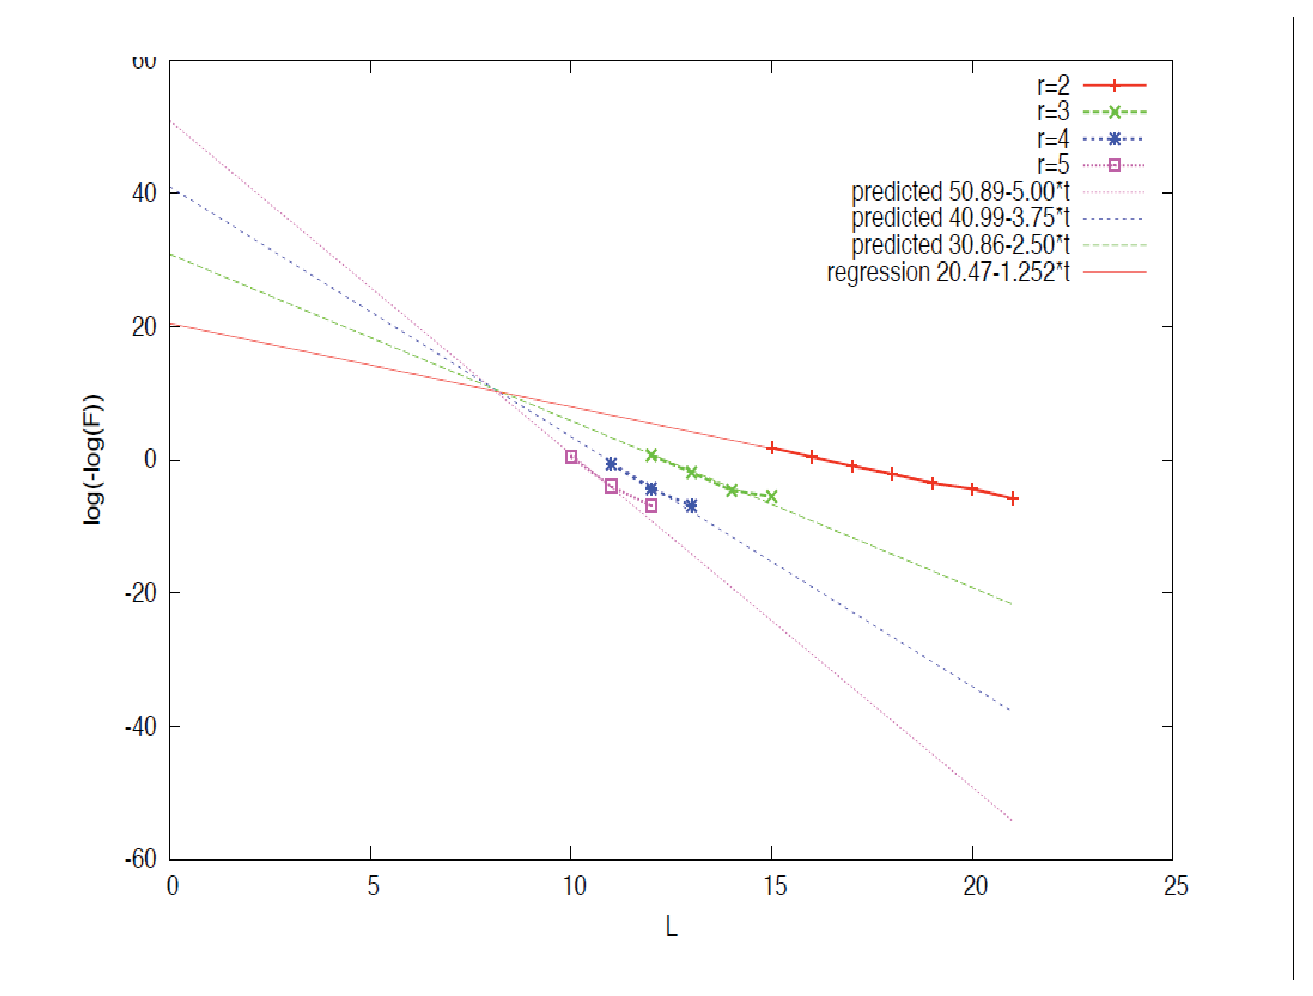
\epsfig{file=./figures/exactseeds.eps,width=4.5in}
\caption{First test, Exact Seeds. We generated 1000 random sequence of size $10^{5}$bp with GC = 0.6. For each sequence,
we detected the longest 2-copy, 3-copy, ..., 5-copy repeat. Using all sequences, we then generated the F
cumulative distribution and plotted it as a function of t (here the seed length). Results
are shown in figure 1 (dots with line r = 2, r = 3, ...). Using the multiplicity r = 2, we
estimated both K = 1.5527 and p = 0.2859.}

\label{fig-hmm}\vspace{-0.2cm}
\end{figure}
\subsection{From 2-copy to $r$-copy repeats}
We need to generalize this for higher multiplicity, so that we have in there a new term that
is the multiplicity $r$. Basically we can have the exact same reasoning except that this time \textsl{p} is the probability
of having a repeat of multiplicity $r$ and not just 2. It seems reasonable to assume that the
probability of finding a segment of score 1 at positions $i, j, k$ with $0 \leq i < j < k \leq n$ is
$\textsl{p}^{r-1}$. The first position can be anything, all the other ones have to be similar segments.
Moreover, we also need to find how many arrangement we can have with more than 2
copies. This is rather easy since if we have $r$ copies in a sequence of length $n$. If we have
$l-{rep}\ll n$, we can ignore the border effect and then we have $(_{2}^\textsl{n})$
possible positions. Therefore we can express the more general form as:

\begin{equation}
\textsl{P}(score \geq t|r) \approx 1-e^{(\textsl{K}(_{r}^\textsl{n})\textsl{p}^{(r-1)t})}
\end{equation}

This equation, using the same transformation as for 2-copy repeats, can be expressed as:

\begin{equation}
\log(-\log(\textsl{F}))= \log(\textsl{K})+\log((_{r}^\textsl{n}))+t(r-1)\log(\textsl{p})
\end{equation}

If this is true, it means that one can estimate only the parameters \textsl{K} and \textsl{p} once
for multiplicity 2 and then have the relationship between scores and probability for all
multiplicities. In practice this means that it becomes feasible and that we do not need to
find all $\textsl{K}_{r}$ and $\textsl{p}_{r}$ by simulation with $r \in [2,\inf]$.



\subsection{What's next?}
Well, it seems that the method I proposed above (maybe others have been using the same
trick) works for strict repeats. Let�s test it for non-strict repeats.

\section{Results}

%describe and present results(table)
%\begin{comment}

%\begin{table}[b]
%\scriptsize
%  \centering
%\begin{tabular}{|c|rcccc|}
%\hline Pattern & Program & Sn \% & Sp \% & T (s) & Sw \\
%\hline
%    & EulerAlign     &??? & ??? & 9 & - \\
%  1 & HomologMiner  &??? & ??? & 9 & - \\
%   &  procrastAlign  &??? & ??? & 9 & - \\
%
%\hline
%\end{tabular}
%\vspace{0.1cm}
% \label{tab-results}
%  \caption{}
%
%\end{table}

We have previously demonstrated the sensitivity of our chaining method in finding Alu repeats in
the human genome~\cite{ref-procrast}. Figure~\ref{fig-align} shows an example local multiple alignment of an ALU family as generated with \texttt{procrastAligner}. To highlight the benefits of our proposed heuristic for gapped extension, we compare \texttt{procrastAligner}'s performance to that of two related programs, EulerAlign~\cite{ref-related1} and HomologMiner~\cite{ref-homologminer}. For this comparison we have inserted mutated copies of randomly generated patterns into the complete genome of \emph{Mycoplasma genitalium}. \emph{M. genitalium} has been recognized as a complex and repeat rich genome, presenting a biologically relevant and challenging example to evaluate our method~\cite{ref-mycoplasma}. We generated and inserted DNA patterns into the genome as follows. To evaluate sensitivity and specificity of the methods as a function of multiplicity we generated 10 patterns for each multiplicity between 2 and 300. To generate each pattern, we first randomly determined a length for each multiplicity (larger pattern lengths for lower multiplicities and vice versa) using the following exponential equation: $l = 200e^{-0.01r}$ , where $r$ is pattern multiplicity and $l$ the calculated length. Next, we constructed the DNA pattern by using a background nucleotide frequency equivalent to the composition of \emph{Mycoplasma genitalium} ($A=0.34,T=0.34,G=0.16,C=0.16$). Then, we randomly mutated each copy of the pattern following a star tree topology. Some positions in the pattern were taken to be more likely to contain mutations by using a gamma-distributed rate heterogeneity. The distance between each mutation and length of indels were calculated using a Poisson distribution. Sequence divergence was varied from 0 substitutions per site (i.e. no divergence) to 1 substitution per site, allowing us also to analyze sensitivity and specificity of each method as a function of sequence divergence. Afterwards, we assigned an orientation to each copy by selecting either the forward or reverse strand.

Now that the pattern and all copies are ready to be inserted into the sequence, we randomly selected the minimum distance between any two copies (between 100-1000nt) following a uniform distribution and inserted each copy into the genome.  We started the analysis by simply recording each method's ability to recover all mutated copies of the  artificially generated pattern. If a copy of the pattern was found, it was recorded as a hit, else miss. We also used each method to find all significant multiple local alignments in the modified genome of \emph{M. genitalium} and recorded their respective sensitivity and specificity as a function of multiplicity and sequence divergences. Results of this experiment are reported in Table~\ref{tab-results}. Parameters used for each program were configured as follows: \\ \\ \textbf{procrastAligner}:\texttt{--z=9 --w=30 --solid=0 --chain=1 --extend=1}\\ \textbf{EulerAlign}:\texttt{ -k 9 -l -i 50 -v} \\ \textbf{HomologMiner}:\texttt{M=20 C=200 T=15 S=10}.


\begin{figure}[t]
\centering 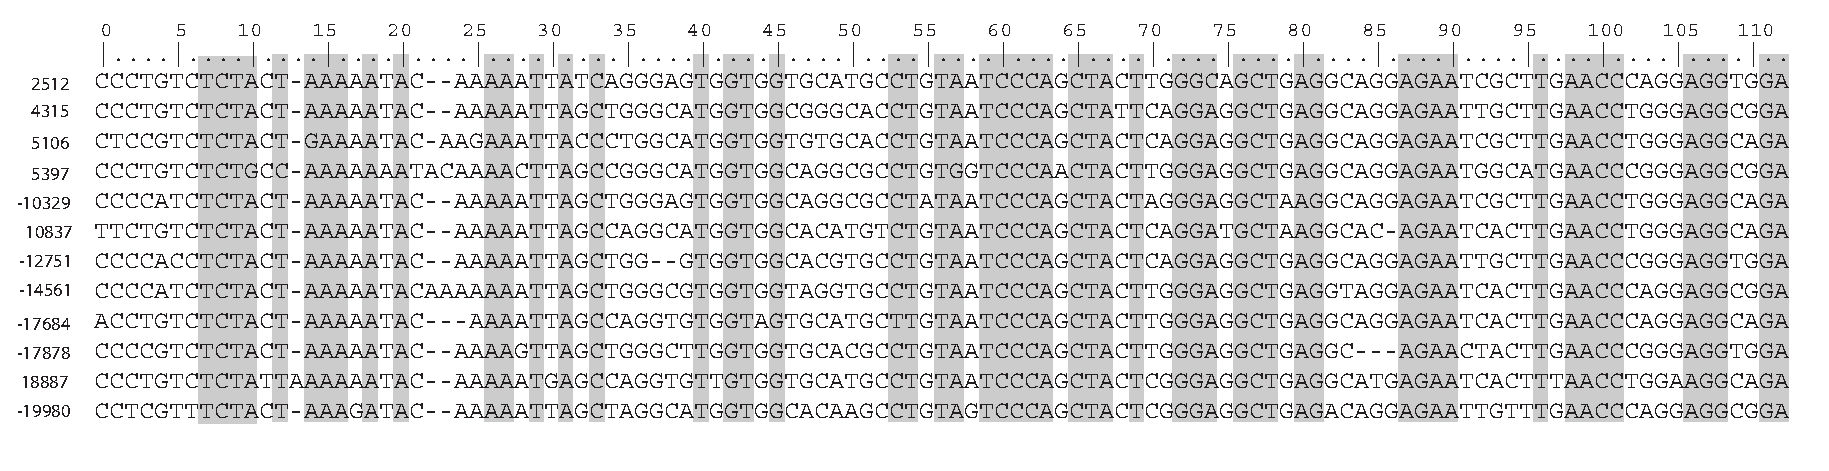
\epsfig{file=./figures/alu_align.eps,width=4.5in}
\caption{Partial alignment of Alu-Sc subfamily found in \emph{H. sapiens} C1 esterase inhibitor gene. Each row represents an aligned ALU. Highlighted columns indicate conserved sequence among all all 10 sequences.}
\label{fig-align}
\end{figure}

\section{Discussion}

We have presented a sensitive and efficient heuristic for local multiple alignment.
We have extended previous results by converting chains of ungapped alignments into to multiple local alignments. We do so via a novel heuristic for directly computing local multiple alignments that utilizes the MUSCLE multiple alignment algorithm to compute gapped extensions of seed matches.  Our method assumes that a fixed number of nucleotides flanking a seed match is likely to be homologous and computes a global multiple alignment on the flanking region.  In some cases our assumption of flanking homology proves erroneous and results in an alignment of unrelated sequences.  We apply random walk statistics to detect any such non-homologous regions embedded in the global multiple alignment.
Present results have demonstrated both high sensitivity and specificity on aligning Alu
sequences and retrieving multiple copies of mutated patterns. We have also presented a statistic method for assigning significance to the resulting multiple local alignments that is used to select only the highly significant alignments.While we view the statistical significance proposal a preliminary, thus far the results of our significance assessment indicates a promising avenue of further research.

\section{Implementation}
We have implemented our method in a program, \texttt{procrastAligner}, available for Linux, Windows, and Mac OS X. Our open-source implementation is available as C++ source code licensed under the GPL.

\section{ Acknowledgments }
AED was supported by NSF grant DBI-0630765. TJT was
supported by Spanish Ministry MECD Grant TIN2004-03382 and AGAUR
Training Grant FI-IQUC-2005.


\bibliographystyle{ws-procs9x6}
\bibliography{procrastination}

\end{document}
